\documentclass[12pt,letterpaper]{article}
%\usepackage{fullpage}
\usepackage[top=2cm, bottom=4.5cm, left=2.5cm, right=2.5cm]{geometry}
\usepackage{amsmath,amsthm,amsfonts,amssymb,amscd}
%\usepackage{lastpage}
\usepackage{enumerate}
\usepackage{fancyhdr}
%\usepackage{mathrsfs}
\usepackage{xcolor}
\usepackage{graphicx}
\usepackage{listings}
\usepackage{hyperref}
\usepackage{float}

\hypersetup{%
  colorlinks=true,
  linkcolor=blue,
  linkbordercolor={0 0 1}
}
 
\renewcommand\lstlistingname{Code}
\renewcommand\lstlistlistingname{Code}
\def\lstlistingautorefname{Alg.}

\lstdefinestyle{C}{
    language        = C,
    frame           = lines, 
    basicstyle      = \footnotesize,
    keywordstyle    = \color{blue},
    stringstyle     = \color{green},
    commentstyle    = \color{red}\ttfamily
}

\setlength{\parindent}{0.0in}
\setlength{\parskip}{0.05in}

% Edit these as appropriate

\pagestyle{fancyplain}
\headheight 35pt
\lhead{Rahul Wankhede \\ MTech (Res), CDS}                 % <-- Comment this line out for problem sets (make sure you are person #1)
\chead{\textbf{\Large OpenMP Assignment}}
\rhead{DS 288 \\ Due: Nov 17th, 2019}
\lfoot{}
\cfoot{}
\rfoot{\small\thepage}
\headsep 1.5em

\begin{document}

\section{Methodology}

Histogram calculation function is a simple for loop that takes the array and histogram array as inputs and fills the histogram array according to the number seen from the array that we generated.

 
\subsection{Serial implementation}

Pretty self-explanatory. 

\subsection{OpenMP implementation}

\subsubsection{Locks}

Tried using locks to lock the interval before incrementing its count and then releasing after it's done. This gives a time that is actually more than the serial implementation. In fact, it performs around 50x worse than the simple serial implementation. This could be due to the fact that there are a very few intervals, which means a lot of contention for locks. Maybe this implementation could've worked well if we had a lot of intervals (in the thousands, perhaps).

\subsubsection{Temporary local histogram array per thread}

So we give a private array to each thread to increment its count on, so there is no contention between threads. When it's done, we add the temporary arrays together in a critical section. This should be fine since the code in the critical section is small.

\section{Experimental Setup}

Using an int array of length $2^{32}$

So, size = $2^2 \times 2^{30} \times 4$B

= 16 GB

the maximum size that I found the machine could allocate on the heap.

Loading the array with $2^{32}$ values between 1 and 20 with seed=10

Using clock\_gettime() function from the time.h library for more detailed timing and timing only the time spent in the histogram function.

\section{Results}
The correctness can be checked by looking at the output files and observing that the times are same for serial and parallel implementations regardless of the number of threads.

\subsection{Serial Results}

The serial implementation took time (in milliseconds) as seen in the table:

\begin{center}
\begin{tabular}{c c c c c c c}
\hline
Interval size	&	1		&	2		&	3		&	4		&	5 		& Average	\\
\hline
1				&	24710	&	24674	& 	24792	&	24871	&	24710 	&	24751 \\
2				&	24447	&	24633	&	24557	&	24461	&	24447 	&	24509 \\
4				&	24489	&	24679	&	24603	&	24691	& 	24489 	&	24590 \\
5				&	24636	&	24498	&	24537	&	24670	&	24636 	&	24535 \\
10				&	24482	&	24695	&	24671	&	24758	&	24482 	&	24617 \\
\hline
\end{tabular}
\end{center}

Average time = \textbf{24.6} seconds (regardless of interval size)

\subsection{Parallel results}

\subsubsection{Threads=2}

\begin{center}
\begin{tabular}{c c c c c c c}
\hline
Interval size	&	1		&	2		&	3		&	4		&	5 		& Average	\\
\hline
1				&	15210	&	14338	& 	14577	&	14430	&	14348 	&	14580 \\
2				&	14570	&	14417	&	14434	&	14373	&	14420 	&	14442 \\
4				&	14331	&	14375	&	14586	&	14376	& 	14613 	&	14456 \\
5				&	14569	&	14395	&	14376	&	14526	&	14441 	&	14461 \\
10				&	14558	&	14440	&	14521	&	14465	&	14621 	&	14521 \\
\hline
\end{tabular}
\end{center}

Average time taken with 2 threads = \textbf{14.5} seconds (regardless of interval size)

Speedup = 1.7x

\newpage

\subsubsection{Threads=4}

\begin{center}
\begin{tabular}{c c c c c c c}
\hline
Interval size	&	1		&	2		&	3		&	4		&	5 		& Average	\\
\hline
1				&	9259	&	9356	& 	9119	&	9449	&	9253 	&	9287\\
2				&	8970	&	9257	&	9193	&	9454	&	9348 	&	9244\\
4				&	9262	&	9439	&	8894	&	9447	& 	9246 	&	9257\\
5				&	9235	&	9403	&	12154	&	9251	&	8997 	&	9808\\
10				&	9458	&	9137	&	9368	&	9292	&	9194 	&	9289\\
\hline
\end{tabular}
\end{center}

Average time taken with 4 threads = \textbf{9.3} seconds

Speedup = 2.6x

\subsubsection{Threads=8}

\begin{center}
\begin{tabular}{c c c c c c c}
\hline
Interval size	&	1		&	2		&	3		&	4		&	5 		& Average	\\
\hline
1				&	9333	&	9427	& 	9146	&	10774	&	8657 	&	9467\\
2				&	9632	&	10205	&	9066	&	8352	&	10011 	&	9453\\
4				&	9196	&	10393	&	7594	&	8455	& 	9365	&	9000\\
5				&	8702	&	7570	&	9072	&	10334	&	9620 	&	9059\\
10				&	9655	&	9410	&	11163	&	10922	&	10762 	&	10382\\
\hline
\end{tabular}
\end{center}

Average time taken with 8 threads = \textbf{9.2} seconds

Speedup = 2.7x


\subsubsection{Threads=16 and onwards}

The maximum number of threads that one node on the cluster can provide is 8. We can still go upto 16 threads by virtue of hyperthreading, but not beyond that. So we'll stick with 8 threads as maximum.

\newpage

\section{Observations}


For an increasing number of threads, we observe a not-so-linear increase in speedup.


\begin{figure}[H]
\centering
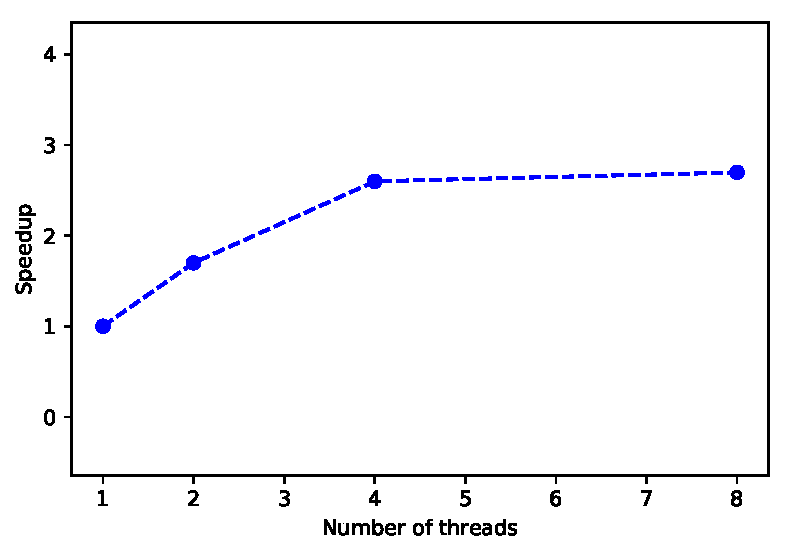
\includegraphics{./vssplot}
\caption{Average speedup obtained for different number of threads}
\end{figure}

\end{document}
